\documentclass[10pt,twocolumn,letterpaper]{article}

\usepackage{cvpr}
\usepackage{times}
\usepackage{epsfig}
\usepackage{graphicx}
\usepackage{amsmath}
\usepackage{amssymb}
\usepackage{gensymb}

% Include other packages here, before hyperref.

% If you comment hyperref and then uncomment it, you should delete
% egpaper.aux before re-running latex.  (Or just hit 'q' on the first latex
% run, let it finish, and you should be clear).
%\usepackage[pagebackref=true,breaklinks=true,letterpaper=true,colorlinks,bookmarks=false]{hyperref}

\cvprfinalcopy % *** Uncomment this line for the final submission

\def\cvprPaperID{****} % *** Enter the 3DV Paper ID here
\def\httilde{\mbox{\tt\raisebox{-.5ex}{\symbol{126}}}}

% Pages are numbered in submission mode, and unnumbered in camera-ready
%\ifcvprfinal\pagestyle{empty}\fi
\setcounter{page}{1}
\begin{document}

%%%%%%%%% TITLE
\title{Omni-directional stereo for 360$\degree$ 3D virual reality video}

\author{Prashanth Chandran\\
ETH Zurich\\
www.ethz.ch\\
{\tt\small chandranp@student.ethz.ch}
% For a paper whose authors are all at the same institution,
% omit the following lines up until the closing ``}''.
% Additional authors and addresses can be added with ``\and'',
% just like the second author.
% To save space, use either the email address or home page, not both
\and
Sasha Pagani\\
ETH Zurich\\
www.ethz.ch\\
{\tt\small paganis@student.ethz.ch}
\and
Julia Giger\\
ETH Zurich\\
www.ethz.ch\\
{\tt\small jgiger@student.ethz.ch}
}

\maketitle
%\thispagestyle{empty}

%%%%%%%%% ABSTRACT
\begin{abstract}
   This project is an implementation of an Omni directional stereo (ODS) renderer called 'Jump' that was proposed by Anderson et.al in \cite{jump16}.  
\end{abstract}

%%%%%%%%% BODY TEXT
\section{Introduction}

An ideal virtual reality environment is one where the user can experience the world in 1) stereo, where eye get an image appropriate to where the user is sees, and 2) in 360 degrees, where the user is free to look in any direction. The rendering of Omni directional stereo content is therefore absolutely necessary for visual immersion. 

The perception of depth in human stereo or binocular vision is a result of the fusion of images captured by the left and right eyes. 
In order to render stereo images, we need to capture synchronized frames from two cameras set apart by the interpupillary distance (IPD); which denotes the distance between our two eyes. The IPD on average about 6.4 cm. However, since for applications in virtual reality, we not only require images that are rendered in stereo, but for them to also be omni-directional. 

One straight forward method of capturing such videos in 360 would be to use two omni-directional cameras that are separated by the human IPD. This method however, suffers from two limitations. The first problem with such an approach is that the two cameras would see each other. The second and more important problem is that the objects which lie on the line passing through the two camera centers will have no disparity (see figure~\ref{two_360}). The absence of disparity makes the perception of depth impossible and therefore, with this simple solution, we would not be able to render  videos in omni-directional stereo.

Ideally, what we want is to have a stereo image pair for every orientation of the head (see figure~\ref{wanted}). This would result in the capture of a huge number of images. Instead, if we could capture only the central ray from each camera and borrow other rays from the central rays of neighbouring camera positions, we could greatly reduce the number of images we need(see figure~\ref{approx}). Figure~\ref{ods} illustrates the extension of this approach to 360$\degree$.

This report is organized as follows. In section \ref{related-work}, we discuss related work and highlight the contributions of \cite{jump16}. Section \ref{work-division} describes how the work was split among the members of our team. Section \ref{method} describes our implementation of the ODS stitching pipeline in detail. In section \ref{results}, we present the results obtained using our renderer and in section \ref{discussion}, we discuss its advantages and shortcomings. Our contributions are summarized in section \ref{conclusion}.

\begin{figure}[t]
\begin{center}
   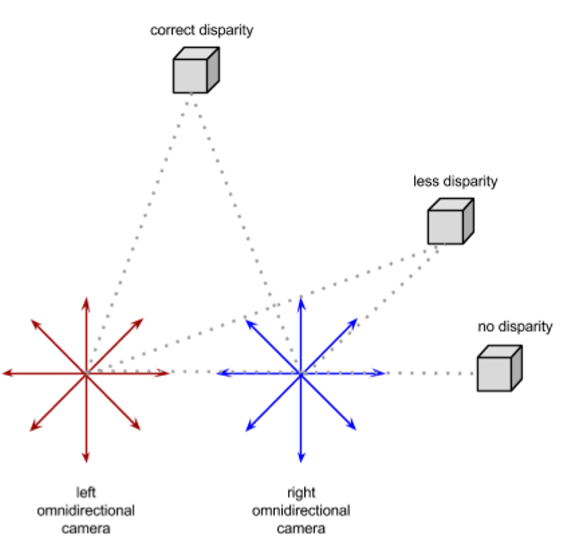
\includegraphics[width=0.8\linewidth]{pictures/two_360.png}
\end{center}
   \caption{Illustration of two 360$\degree$ cameras placed next to each other.}
\label{two_360}
\end{figure}

\begin{figure}[t]
\begin{center}
   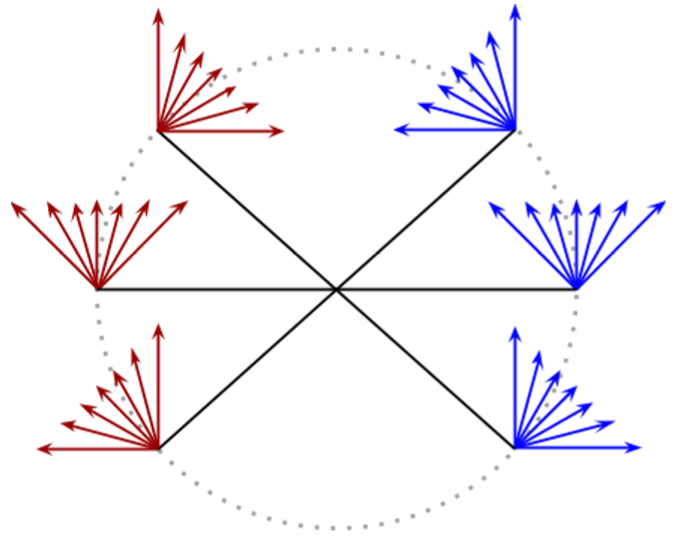
\includegraphics[width=0.5\linewidth]{pictures/wanted.png}
\end{center}
   \caption{This image shows the most optimal situation, where a full image is captured for each head direction. The red rays illustrate the left eye and the blue ones the left eye.}
\label{wanted}
\end{figure}

\begin{figure}[t]
\begin{center}
	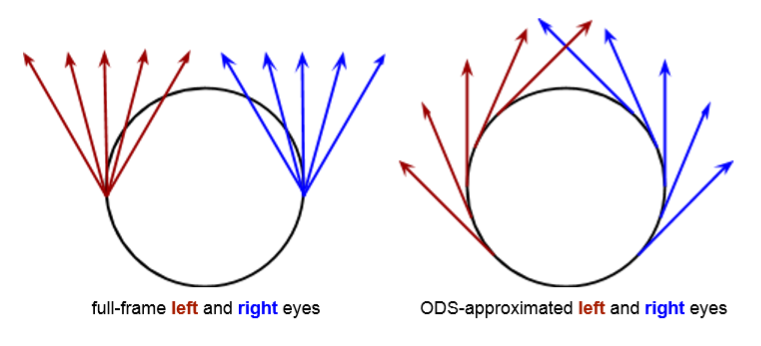
\includegraphics[width=0.8\linewidth]{pictures/approxi.png}
\end{center}
   \caption{The left image shows the rays for capturing the full image at one head direction. The right image illustrates the ODS approximation by using only the central ray of each camera position.}
\label{approx}
\end{figure}

\begin{figure}[t]
\begin{center}
   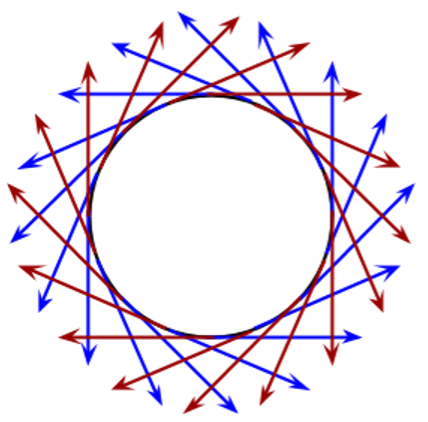
\includegraphics[width=0.5\linewidth]{pictures/ods.png}
\end{center}
   \caption{This image shows the ODS approximation for 360$\degree$. The red rays illustrates the left eye and the blue rays the right eye.}
\label{ods}
\end{figure}


%------------------------------------------------------------------------
\section{Related work}
\label{related-work}
Several methods in the past have been proposed to tackle the problem of rendering omni directional stereo content. We discuss two such methods that are particularly interesting. 'Omnistereo: Panaromic stereo imaging', proposed in \cite{peleg}, described the multiple view point projection involved in the generation of omni-directional stereo images. The authors used a single rotating camera to capture images in 360 degrees. Another approach is 'MegaStereo' \cite{megastereo}. 

Both methods \cite{peleg} and \cite{megastereo}, capture omni-directional panaromas with a single rotating camera. This means that they rely on the scene being static or that there is little motion. In \cite{jump16}, the authors propose a new camera rig with 16 cameras that allows for large scene motion. They also use optical flow based view interpolation to synthesize images between adjacent cameras in the rig. A key contribution of \cite{jump16} is that their view interpolation and composting framework, can generate ODS panaromas from only 16 images, while previous methods like \cite{megastereo} required hundreds of images. 

\subsection{Our implementation of \textit{Jump} \cite{jump16}}
In this project, our goal was to implement the ODS stitching pipeline proposed by Anderson et al.~\cite{jump16}. While staying loyal to main steps of their stitching pipeline, we would like to highlight a few differences in our implementation. The first is that the authors in \cite{jump16}, proposed a new and sophisticated optical flow computation algorithm, that was designed to be optimal for the task of view interpolation in scenes with large motion.  For time constraints, we did not implement the optical flow they proposed and used an off the shelf dense optical algorithm from OpenCV. Furthermore, we simplified the exposure correction and the composition step. For the implementation details, we also used the article~\cite{ods} by Google Inc.

%------------------------------------------------------------------------
\section{Work subdivision}
\label{work-division}
In
%------------------------------------------------------------------------
\section{Method}
\label{method}
An overview of our pipeline can be found in figure~\ref{pipeline}. The inputs are 10 synchronized videos from a camera rig. The first step is the calibration of the different cameras of the rig, which includes the computation of the intrinsics and extrinsics of each camera. The next step is the optical flow estimation between the neighboring camera pairs. For having nice transitions in the final ODS stitch, an exposure correction between neighboring image pairs is applied. Based on the computed flow values, the view interpolation between the images is calculated and they are stitched together as a final step, which results in the desired ODS video.

\begin{figure}[t]
\begin{center}
   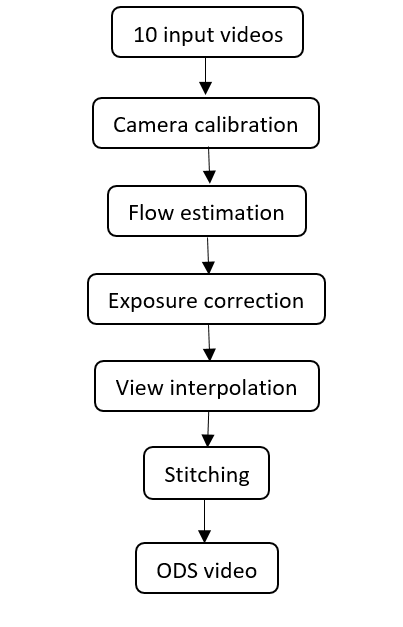
\includegraphics[width=0.3\linewidth]{pictures/pipeline.PNG}
\end{center}
   \caption{Overview of the pipeline.}
\label{pipeline}
\end{figure}

\subsection{Camera calibration}
Additionally to the dataset, consisting of 10 videos, we received a calibration file from our supervisor, which contained the calibration data for each camera. This calibration data consists of the intrinsic and relative extrinsic of each camera. For the computation in the later stages of our pipeline, we also needed the absolute extrinsics of each camera, which were computed with the following formula:
$E_i= E_{i-1} \cdot T_i^{-1}$ where $E_i$ represents absolute extrinsics (relative to camera 0) of camera i while $T_i$ represents the relative extrinsics (with respect to the previous camera) of camera i.

\begin{figure}[t]
\begin{center}
   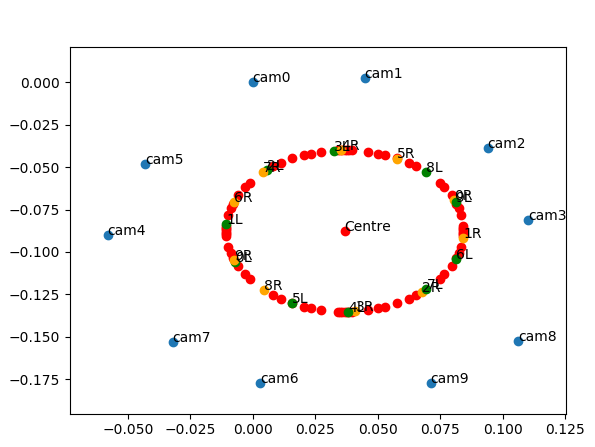
\includegraphics[width=0.8\linewidth]{pictures/our_camera_rig.PNG}
\end{center}
   \caption{An illustration of our camera rig based on the calibration file.}
\label{rig}
\end{figure}

\subsection{Flow estimation}
We did not implement such a sophisticated flow estimation algorithm as in Anderson et al.~\cite{jump16}. Instead, we used an existing per-pixel flow computation method from the OpenCV library.

\subsection{Exposure correction}
For the exposure correction, we interpolate linearly between the average image intensity of the neighboring image pairs:\\
\\
$g_{c}=\dfrac{(\theta_{c}-\theta_{0})}{(\theta_1-\theta_{0})}*g_{0} + \dfrac{(\theta_{1}-\theta_{c})}{(\theta_1-\theta_{0})}*g_{1}$
\\
\subsection{View interpolation}
The main idea of the stitching process is to interpolated between two neighboring images.
We used the following interpolation from Anderson et al.~\cite{jump16} for our view interpolation:\\
\\
$\theta_p=\dfrac{(\theta_{b}-\theta_{1})*\theta_{0}+(\theta_{0}-\theta_{a})*\theta_{1}}{\theta_{b}-\theta_{a}+\theta_{0}-\theta_{1}}$
\\
\\
Where $\theta_ {0}$ and $\theta_ {1}$ are the headings of the two cameras in the ODS stitch. $\theta_ {a}$ is the heading of a point in the first camera and $\theta_ {b}$ is the heading of the same point in the second camera (see figure\ref{interpolation}).

\begin{figure}[t]
\begin{center}
   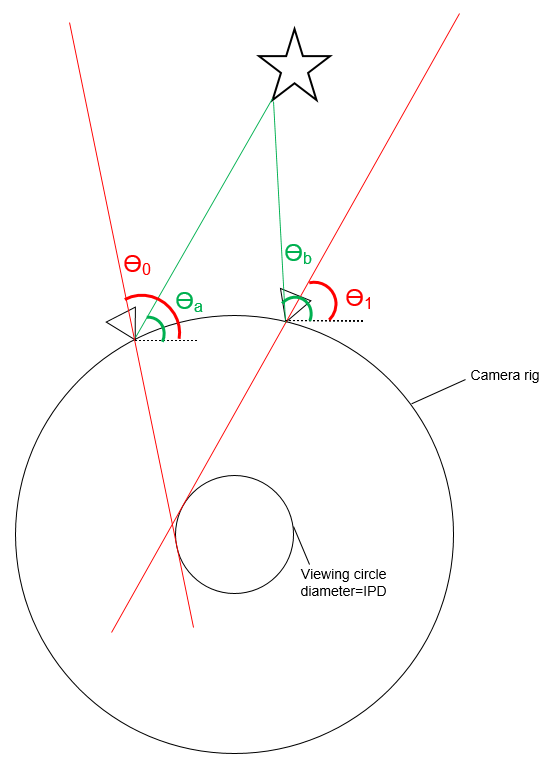
\includegraphics[width=0.7\linewidth]{pictures/interpolation.PNG}
\end{center}
   \caption{This is an illustration of the different angles used in the interpolation formula. The red lines are the central rays of the corresponding camera.}
\label{interpolation}
\end{figure}

\subsection{Stitching}



%------------------------------------------------------------------------
\section{Results}
\label{results}
For testing our implementation we used a dataset provided from our supervisor It's obtained from 10 cameras disposed on an ellipse approaching a circle, which are pairwise equidistant. The calibration file was provided too. For getting an idea of the possible output, we produced an homography stitching which can be seen in image ...
In Figure ~\ref{lefteye} we can instead see the output of the ODS stitching for our dataset for the left eye considering the first frame.
\begin{figure}[t]
\begin{center}
   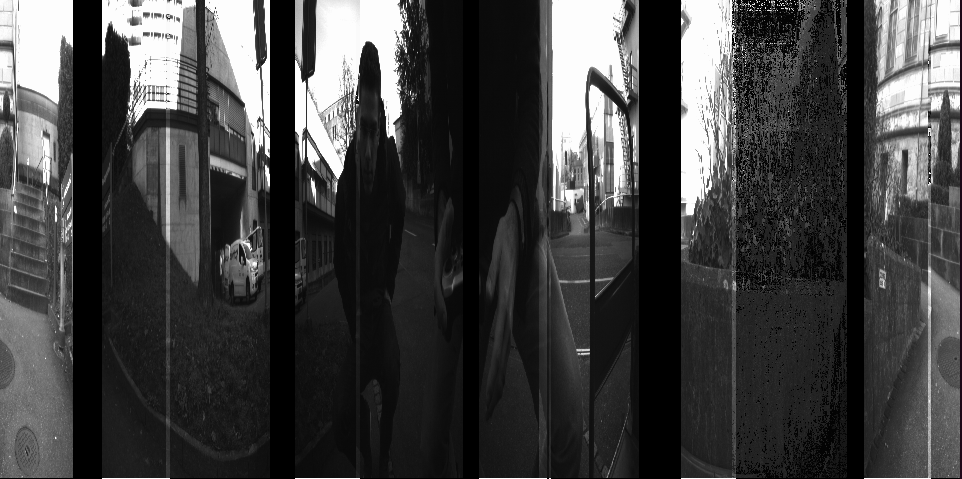
\includegraphics[width=0.7\linewidth]{pictures/frame0_lefteye_cwise.png}
\end{center}
   \caption{ODS stitching result for the left eye, first frame.}
\label{lefteye}
\end{figure}

%------------------------------------------------------------------------
\section{Discussion}
\label{discussion}
As we can see in picture ~\ref{lefteye} we get good results only for the camera couples which provide a good overlap. This is due to the fact that the optical flow between the other images is very low since they don't have much in common. Another issue is that if we take a look at the image planes plotted in Figure ~\ref{imageplanes} there are empty spaces between them. For this we don't have a real idea of why it happens, it could be because of problems with the calibration file.
Further, better results could have been obtained if we had an Odyssey GoPro at disposal since this would have given us the same working conditions as the authors had.
\begin{figure}[t]
\begin{center}
   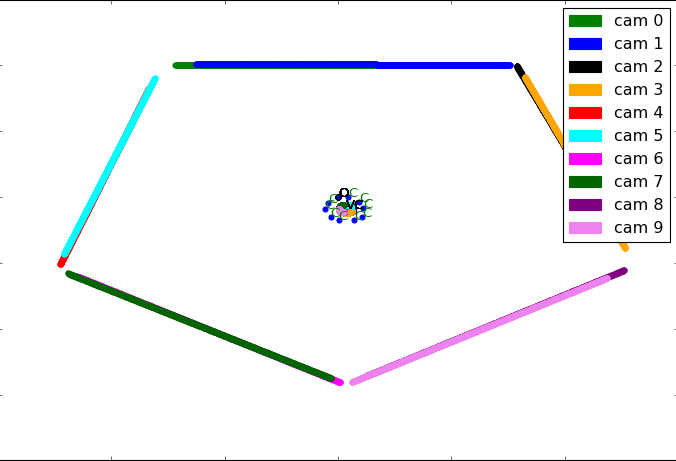
\includegraphics[width=0.7\linewidth]{pictures/rig_detailed.png}
\end{center}
   \caption{Plot of the image planes of the different cameras}
\label{imageplanes}
\end{figure}
%------------------------------------------------------------------------
\section{Conclusion}
\label{conclusion}
The results obtained from Anderson et al.~\cite{jump16} are better than ours but this was expected. We had less cameras at disposal (10 instead of 16) which weren't in a perfect rig like it's the case using the Odyssey GoPro. This would have produced in general a better overlap among the images, which would have resulted in a better interpolation.

{\small
\bibliographystyle{ieee}
\bibliography{egbib}
}

\end{document}
